\documentclass[xcolor=table,10pt,final]{beamer}
\renewcommand\mathfamilydefault{\rmdefault}

\setbeamertemplate{navigation symbols}{}
\usepackage{amsmath,amsfonts,amssymb,pxfonts,xspace}
\usepackage{textcomp}
\usepackage{lmodern}
\usepackage{verbatim}
\usepackage{graphicx}
\usepackage{listings}
\usepackage[T1]{fontenc}

\lstset{
    language=Python,
    basicstyle=\footnotesize,
    keywordstyle=\color[rgb]{0.1,0.8,0.1}\bfseries,
    commentstyle=\color{blue},
    numbers=left,
    stringstyle=\ttfamily\color{red!50!brown},
    showstringspaces=false}
\lstset{literate=%
   *{0}{{{\color{red!20!violet}0}}}1
    {1}{{{\color{red!20!violet}1}}}1
    {2}{{{\color{red!20!violet}2}}}1
    {3}{{{\color{red!20!violet}3}}}1
    {4}{{{\color{red!20!violet}4}}}1
    {5}{{{\color{red!20!violet}5}}}1
    {6}{{{\color{red!20!violet}6}}}1
    {7}{{{\color{red!20!violet}7}}}1
    {8}{{{\color{red!20!violet}8}}}1
    {9}{{{\color{red!20!violet}9}}}1
}

\begin{document}
\definecolor{navy}{RGB}{0,0,128}


\title{Python for Scientific Computing}
\subtitle{Lecture 4: Code Improvement}
\author{{\bf Esteban Meneses}\\emeneses@pitt.edu\\{\em Center for Simulation and Modeling (SaM)}}
\date{\today}
\frame{\titlepage}

\begin{frame}
	\frametitle{What does Code Improvement mean?}
	\begin{itemize}
		\item Algorithm Design
		\begin{itemize}
			\item Iteration vs recursion
			\item Number of operations
		\end{itemize}
		\item Profiler
		\item Debugger
	\end{itemize}
\end{frame}

{\setbeamercolor{background canvas}{bg=navy}
\begin{frame}
	\frametitle{\textcolor{yellow}{Exercise 1}}
	\textcolor{white}{Write a Python function to compute the \emph{n-th Fibonacci} number.\newline\newline
	 {\tt fibonacci(0) = 0\\
	 fibonacci(1) = 1\\
	 fibonacci(n) = fibonacci(n-1) + fibonacci(n-2)}
	}
\end{frame}
}

\begin{frame}
	\frametitle{Recursive Fibonacci function}
	\begin{itemize}
		\item x
	\end{itemize}
\end{frame}

\begin{frame}
	\frametitle{y}
	\begin{itemize}
		\item x
	\end{itemize}
\end{frame}

\begin{frame}
	\frametitle{Recursion in Hollywood}
	\begin{columns}[t,totalwidth=\textwidth]
		\begin{column}{.7\linewidth}
			\\
			\vspace{-2.0cm}
			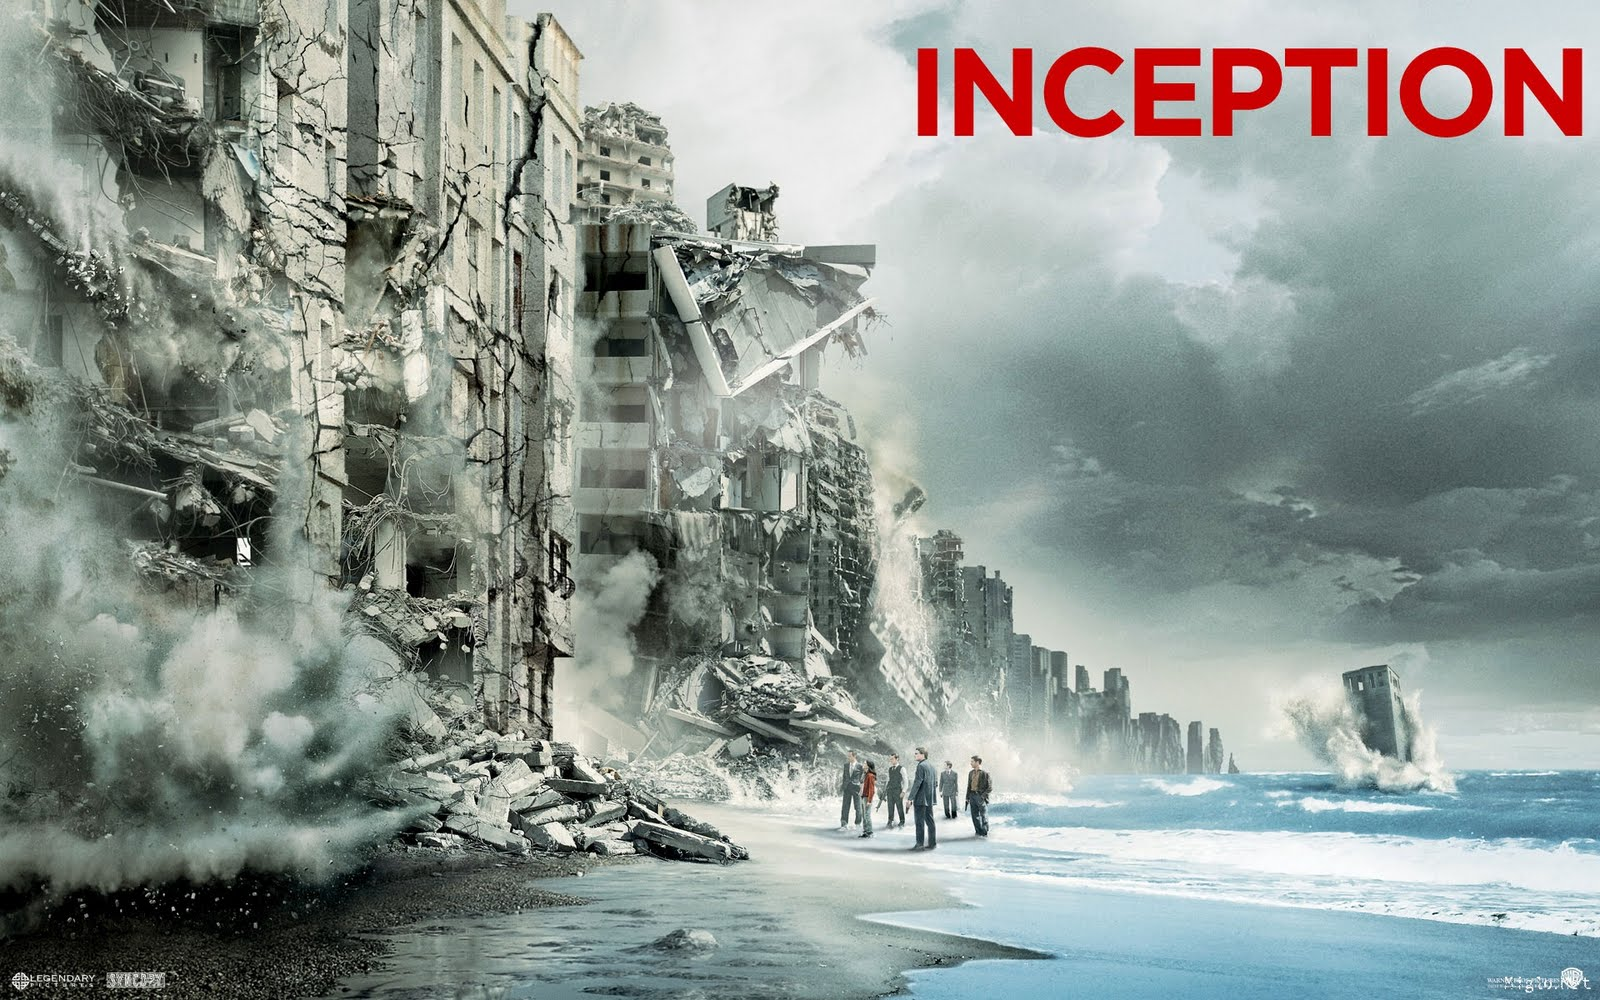
\includegraphics[scale=0.12]{inception}
		\end{column}
		\begin{column}{.3\linewidth}
			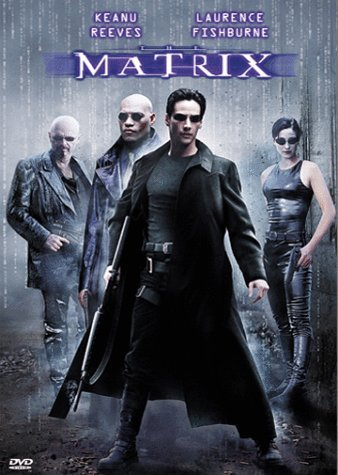
\includegraphics[scale=0.2]{matrix}\\ \vspace{0.5cm}
			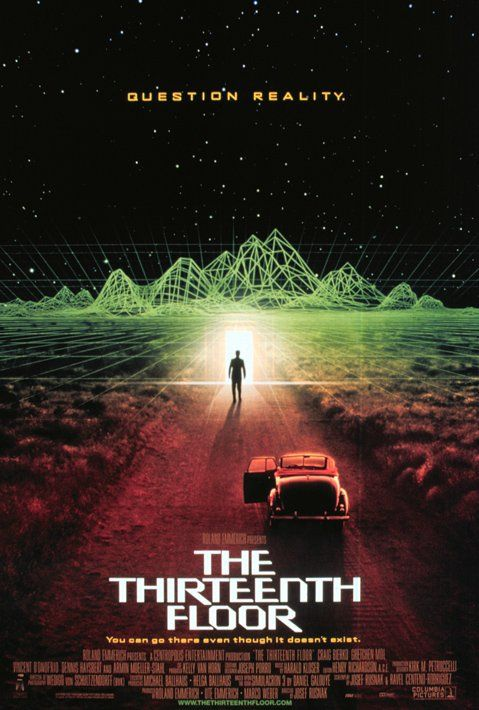
\includegraphics[scale=0.14]{floor}			
		\end{column}
	\end{columns}
\end{frame}

\begin{frame}
	\frametitle{y}
	\begin{itemize}
		\item x
	\end{itemize}
\end{frame}

\begin{frame}
	\frametitle{y}
	\begin{itemize}
		\item x
	\end{itemize}
\end{frame}

{\setbeamercolor{background canvas}{bg=navy}
\begin{frame}
	\frametitle{\textcolor{yellow}{Exercise 2}}
	\textcolor{white}{Write a Python function to sort a list of integers using the \emph{bubble sort} algorithm.\newline\newline
	 {\tt gcd(x,y) = }
	}
\end{frame}
}

\begin{frame}
	\frametitle{y}
	\begin{itemize}
		\item x
	\end{itemize}
\end{frame}

\begin{frame}
	\frametitle{Magic functions in IPython}
	\begin{itemize}
		\item Special commands to modify execution or environment
		\item Examples:
		\begin{itemize}
			\item \%paste
			\item \%run
		\end{itemize}
	\end{itemize}
\end{frame}



\begin{frame}
	\frametitle{y}
	\begin{itemize}
		\item x
	\end{itemize}
\end{frame}

{\setbeamercolor{background canvas}{bg=navy}
\setbeamercolor{itemize item}{fg=yellow}
\begin{frame}
	\frametitle{\textcolor{yellow}{Concluding Remarks}}
	\begin{itemize}
		\item \textcolor{white}{Try a different implementation: recursion $\rightarrow$ iteration.}
		\item \textcolor{white}{Try a different algorithm: reduce number of operations.}
		\item \textcolor{white}{Use the profiler to detect performance bottlenecks.}
		\item \textcolor{white}{Use debugger to hunt down programming errors.}
	\end{itemize}
\end{frame}
}

%\begin{frame}
%	\frametitle{y}
%	\begin{itemize}
%		\item x
%	\end{itemize}
%\end{frame}

\end{document}
